%---------------------------------------------------------

\subsubsection{Pruning Analysis}

% Epsilon can be bad

% Worst case

% Best case
Next, we provide a best-case and worst-case analysis of the amount of pruning obtained when using BAB, when applied to deterministic games. 
The worst-case for classical Alpha-Beta is to explore the entire tree without eliminate any leaf node. For a balanced tree with a branching factor $b$ and depth $d$ this means generating $O(b^d)$ states. In the best-case, however, Alpha-Beta can generate only $\mathcal{O}(b^{d/2})$ \cite{knuth1975analysis}. 


Now, lets examine the nodes that must be expanded by the BAB algorithm. 
For this analysis, let $\vmin=-\infty$ and $\vmax=\infty$. 
Observe that every generate node $n$ must generate at least one of its children $c$. This is because if $n$ has been generated, it means that its parent didn't prune it, i.e., $\alpha(p(n))+\epsilon<\beta(p(n))$. 
Thus, $n$ cannot do any pruning before seeing at least one node. 
We call this child the \emph{left-most child} of $n$,
and we say that a node $n'$ is a left-most descendant of $n$
if $n'$ is a left-most child of a left most-child ... of $n$. 
Clearly all left-most descendant of $\rootnode$ must be expanded. 
Consider the left-most child $c$ of $\rootnode$. 
Since $\alpha(\rootnode)=\vmin$ and $\beta(\rootnode)=\vmax$, 
then also $\alpha(c)=\vmin$ and $\beta(c)=\vmax$. 

Assume that $\rootnode$ is a MAX node. 
It initializes $\alpha(\rootnode)=\vmin$ and $\beta(\rootnode)=\vmax$. 
Generating and solving the children of $\rootnode$


Its 

$n'$ parent and its parent

call every left-most child of 
Assume that $n$ is a MAX node. 
This means that when $n$'s left-most child was generated, 
$\alpha(n)=\alpha(p(n))$ and $\beta(n)=\beta(p(n))$. 
Since $\alpha(\rootnode)=\vmin$ and $\beta(\rootnode)=\vmax$, 
we have that for all left most 

Obviously, the root of the search must be expanded. 

Every generated node must generate at least is left-most child. 


To do so, we assign coordinate numbers to the nodes of the tree as in the "Dewey decimal system" (DDC). In DDC, every node $n$ on level $l$ can be describe by a sequence of integers $(a_1, a_2 \ldots a_l)$, where $a_i$ is the number of a child
that leads to $n$. For example, the sequence $(1, 2, 3)$ describes a node on the tree that can be found by 
moving to the first child from the root, then moving to the second child from that node, and then to the third child. Hence, by DDC the root is described by an empty sequence. 
Lets call a node $(a_1, a_2 \ldots a_l)$ critical if $a_i=1$ for all odd values of $i$ or for all even values of $i$. For example, the nodes $(1, 4, 1, 2, 1), (3, 1, 3, 1), (1, 1), (1, 1, 7, 1, 1, 1, 8, 1, 3, 1, 5)$, and the root are critical.
Lets define a child $c$ of node $n$ as a \emph{bounded~suboptimal~child} if $\MM(n)\in [\pess(c), \pess(c)+\epsilon]$. 

%A node $n$ is examined by BAB if the algorithm is calling $\bab{}(n, \alpha, \beta)$ and $\alpha + \epsilon < \beta$.


\begin{theorem}
 For a game tree $G$ for which the first successor of every node is a $\mathit{bounded~suboptimal~child}$ with a bound of $\epsilon$, the BAB algorithm examines precisely the critical nodes of this game tree.
\label{the:newbest}
\end{theorem}
\begin{proof}
Lets divide the critical nodes into three types.

\begin{itemize}
  \item Type 1: critical node $a_1, a_2 \ldots a_l$ in which $a_i=1$ for all $1 \leq i \leq l$. e.g. $111, 1, 1111$.
  
  \item Type 2: critical node $a_1, a_2 \ldots a_l$ in which $a_i=1$ for all $1 \leq i \leq j-1, a_j>1$, and $l-j$ is even. e.g. $1214, 411, 114$.
  
  \item Type 3: critical node $a_1, a_2 \ldots a_l$ in which $a_i=1$ for all $1 \leq i \leq j-1, a_j>1$, and $l-j$ is odd. e.g. $131, 311131, 21$.
\end{itemize}


The following facts are invariants that can be established by induction on the entire tree.

\begin{enumerate}

  \item $\alpha(n)$ and $\beta(n)$ of a type 1 node $n$ are initialized by $\vmin$ and $\vmax$, respectively. The first child of $n$ is also a type 1 node. All other children of $n$ are of type 2, and their $\alpha$ and $\beta$ values are initialized by $\pess(n)$ and $\vmax$ if $n$ is a MAX node and by $\vmin, \opti(n)$, respectively. 
  
  \item The $\alpha$ and $\beta$ values of a type 2 node $n$ is initialized by $\vmin$ and $\beta(n)$ for MIN nodes and by $\alpha(n)$ and $\vmax$ for MAX nodes, respectively. 
  
  examined by calling $v(n) = \bab(n, \vmin, \beta)$ or $v(n) = \bab(n,\alpha, \vmax)$ (for max or min node, respectively), where 
$\vmin < \beta - \epsilon  \leq  v(n)$ and $v(n)  \leq  \alpha + \epsilon < \vmax$. If $n$ is not a terminal node, its  first child $n_1$ is a type 3 node, and its all other children $n_2, n_3 \ldots n_{b(n)}$ are not examined.
 
  \item A type 3 node $n$ is examined by calling $v(n) = \bab(n,\alpha, \vmax)$ or $v(n) = \bab(n, \vmin, \beta)$ (for max or min node, respectively), where
$\vmin < \beta - \epsilon  \leq  v(n)$ and $v(n)  \leq  \alpha + \epsilon < \vmax$. If $n$ is not a terminal node, each of its children $n_1, n_2 \ldots n_{b(n)}$ 
is of type 2, and are all examined by calling $\bab(n_i, \vmin, -\alpha)$ or $\bab(n_i, -\beta, \vmax)$ (if $n_i$ is max or min node, respectively).

\end{enumerate}

\end{proof}








\begin{theorem}
If $\epsilon < \vmax - \vmin$, then for any input and-or tree, there is a worst-case assignment of values to the leaves so that BAB going left to right develops the full tree.
\label{the:worst}
\end{theorem}
\begin{proof}
First, we determine the assignment of values to the leaves by recursively assigning values to nodes in a top down fashion as follows.

\begin{itemize}
  \item For a max node $n$ assigned to value $v$, we assign the $b(n)-1$ first children of $n$ the value $\vmin$, and assign the $b(n)$th child value $v$.
  \item For a min node $n$ assigned to value $v$, we assign the $b(n)-1$ first children of $n$ the value $\vmax$, and assign the $b(n)$th child value $v$.
  \item For a leaf node assigned to value $v$, we just assign the value $v$.
  \item The above rules define the heredity part of the recursion, for the starting case: it suffices to assign the root to any value strictly between $\vmin$ and $\vmax$.
\end{itemize}

The following facts establish by induction that every node on the tree gets the value assigned in the construction.
\begin{itemize}
  \item A leaf node value is the same value assigned to it in the construction.  
  \item Assuming node children values are the assigned values in the construction, max node $n$ children values are $\vmin$ for the $b(n)-1$ first children and $v$ for the $b(n)$th child. Since $v \geq \vmin$, the value of $n$ must be $v$.
    \item Assuming node children values are the assigned values in the construction, min node $n$ children values are $\vmax$ for the $b(n)-1$ first children and $v$ for the $b(n)$th child. Since $v \leq \vmax$, the value of $n$ must be $v$.
\end{itemize}

During the algorithm for each partially expanded node the $\alpha$ and $\beta$ values are $\vmin$ and $\vmax$ respectively.
\begin{itemize}
  \item A max node $n$ updates its $\alpha$ value after each child. Since the assigned value of the $b(n)-1$ first children is $\vmin$, the value of $\alpha$ remains $\vmin$.
  \item A min node $n$ updates its $\beta$ value after each child. Since the assigned value of the $b(n)-1$ first children is $\vmax$, the value of $\beta$ remains $\vmax$.
\end{itemize}
The algorithm commits pruning if $\beta - \alpha \leq \epsilon$. Because $\alpha = \vmin$ and $\beta = \vmax$ for every partially expanded node, pruning will be committed if $\vmax - \vmin \leq \epsilon$. However, $\epsilon < \vmax - \vmin$ and hence no pruning ever occurs
\end{proof}

In Theorem \ref{the:basic} we shown that BAB return a bounded solution, later in this paper we show empirically that the average time takes to find a solution with bound $\epsilon_2$ is shorter than to find a solution with bound $\epsilon_1$, if $\epsilon_2 > \epsilon_1$. In some special cases, although $\epsilon_2 > \epsilon_1$, the ration between the times takes to find the two solutions can be different. 


\begin{figure}
	\centering
	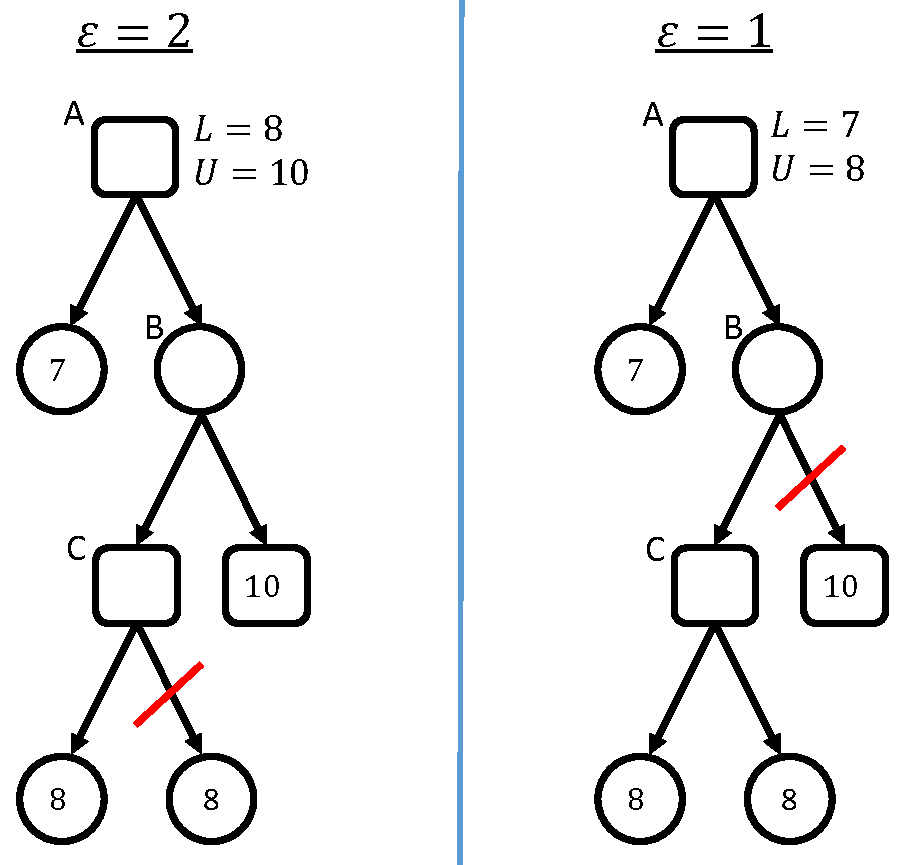
\includegraphics[width=0.8\columnwidth]{Figures/cropped_example_different_e.pdf}
	\caption{Example of BAB pruning}
	\label{fig:bab-prune}
\end{figure}

Figure \ref{fig:bab-prune} demonstrate this phenomenon. The right tree represent an example of BAB with $\epsilon = 1$ and the left one represent BAB with $\epsilon = 2$. In both cases $\vmin = 0$ and $\vmax = 10$. In both cases, after node $A$ explored the left child its $\alpha = 7$ and $\beta = 10$. These values transmitted down to $B$ and from there to $C$. After $C$ explored the left child $\alpha = 8$ and $\beta = 10$. In this point, the left tree prune the right branch and the values that return to $B$ are $(8,10)$, node $B$ update $\beta$ value to $10$ and explore the right child. In the right tree, the right child of $C$ does not get pruned and the values that return to $B$ are $(8,8)$, $B$ update $\beta$ value to $8$ and the right child get pruned. Although these two examples explored the same amount of nodes, the branch of the right child of $B$ and the branch of the right child of $C$ could contain large sub-trees and hence a greater $\epsilon$ value might explore less, more or equal amount of nodes. 


%---------------------------------------------------------
%---------------------------------------------------------




\begin{theorem}
If $\epsilon < \vmax - \vmin$, then for any 
%input and-or tree, 
game tree there is a worst-case assignment of values to the leaves so that BAB will not perform any pruning and 
develop the entire tree. 
%going left to right develops the full tree.
\label{the:worst}
\end{theorem}
\begin{proof}
First, we determine the assignment of values to the leaves by recursively assigning values to nodes in a top down fashion as follows.

\begin{itemize}
  \item For a MAX node $n$ assigned to value $v$, we assign the $b(n)-1$ first children of $n$ the value $\vmin$, and assign the $b(n)$th child value $v$.
  \item For a min node $n$ assigned to value $v$, we assign the $b(n)-1$ first children of $n$ the value $\vmax$, and assign the $b(n)$th child value $v$.
  \item For a leaf node assigned to value $v$, we just assign the value $v$.
  \item The above rules define the heredity part of the recursion, for the starting case: it suffices to assign the root to any value strictly between $\vmin$ and $\vmax$.
\end{itemize}

The following facts establish by induction that every node on the tree gets the value assigned in the construction.
\begin{itemize}
  \item A leaf node value is the same value assigned to it in the construction.  
  \item Assuming node children values are the assigned values in the construction, max node $n$ children values are $\vmin$ for the $b(n)-1$ first children and $v$ for the $b(n)$th child. Since $v \geq \vmin$, the value of $n$ must be $v$.
    \item Assuming node children values are the assigned values in the construction, min node $n$ children values are $\vmax$ for the $b(n)-1$ first children and $v$ for the $b(n)$th child. Since $v \leq \vmax$, the value of $n$ must be $v$.
\end{itemize}

During the algorithm for each partially expanded node the $\alpha$ and $\beta$ values are $\vmin$ and $\vmax$ respectively.
\begin{itemize}
  \item A max node $n$ updates its $\alpha$ value after each child. Since the assigned value of the $b(n)-1$ first children is $\vmin$, the value of $\alpha$ remains $\vmin$.
  \item A min node $n$ updates its $\beta$ value after each child. Since the assigned value of the $b(n)-1$ first children is $\vmax$, the value of $\beta$ remains $\vmax$.
\end{itemize}
The algorithm commits pruning if $\beta - \alpha \leq \epsilon$. Because $\alpha = \vmin$ and $\beta = \vmax$ for every partially expanded node, pruning will be committed if $\vmax - \vmin \leq \epsilon$. However, $\epsilon < \vmax - \vmin$ and hence no pruning ever occurs
\end{proof}







The worst-case for classical Alpha-Beta is to explore the entire tree without eliminate any leaf node. For a balanced tree with a branching factor $b$ and depth $d$ this means generating $O(b^d)$ states. In the best-case, however, Alpha-Beta can generate only $\mathcal{O}(b^{d/2})$ \cite{knuth1975analysis}. 


Now, lets examine the nodes that must be expanded by the BAB algorithm. 
For this analysis, let $\vmin=-\infty$ and $\vmax=\infty$. 
Observe that every generate node $n$ must generate at least one of its children $c$. This is because if $n$ has been generated, it means that its parent didn't prune it, i.e., $\alpha(p(n))+\epsilon<\beta(p(n))$. 
Thus, $n$ cannot do any pruning before seeing at least one node. 
We call this child the \emph{left-most child} of $n$,
and we say that a node $n'$ is a left-most descendant of $n$
if $n'$ is a left-most child of a left most-child ... of $n$. 
Clearly all left-most descendant of $\rootnode$ must be expanded. 
Consider the left-most child $c$ of $\rootnode$. 
Since $\alpha(\rootnode)=\vmin$ and $\beta(\rootnode)=\vmax$, 
then also $\alpha(c)=\vmin$ and $\beta(c)=\vmax$. 

Assume that $\rootnode$ is a MAX node. 
It initializes $\alpha(\rootnode)=\vmin$ and $\beta(\rootnode)=\vmax$. 
Generating and solving the children of $\rootnode$


Its 

$n'$ parent and its parent

call every left-most child of 
Assume that $n$ is a MAX node. 
This means that when $n$'s left-most child was generated, 
$\alpha(n)=\alpha(p(n))$ and $\beta(n)=\beta(p(n))$. 
Since $\alpha(\rootnode)=\vmin$ and $\beta(\rootnode)=\vmax$, 
we have that for all left most 

Obviously, the root of the search must be expanded. 

Every generated node must generate at least is left-most child. 


To do so, we assign coordinate numbers to the nodes of the tree as in the "Dewey decimal system" (DDC). In DDC, every node $n$ on level $l$ can be describe by a sequence of integers $(a_1, a_2 \ldots a_l)$, where $a_i$ is the number of a child
that leads to $n$. For example, the sequence $(1, 2, 3)$ describes a node on the tree that can be found by 
moving to the first child from the root, then moving to the second child from that node, and then to the third child. Hence, by DDC the root is described by an empty sequence. 
Lets call a node $(a_1, a_2 \ldots a_l)$ critical if $a_i=1$ for all odd values of $i$ or for all even values of $i$. For example, the nodes $(1, 4, 1, 2, 1), (3, 1, 3, 1), (1, 1), (1, 1, 7, 1, 1, 1, 8, 1, 3, 1, 5)$, and the root are critical.
Lets define a child $c$ of node $n$ as a \emph{bounded~suboptimal~child} if $\MM(n)\in [\pess(c), \pess(c)+\epsilon]$. 

%A node $n$ is examined by BAB if the algorithm is calling $\bab{}(n, \alpha, \beta)$ and $\alpha + \epsilon < \beta$.


\begin{theorem}
 For a game tree $G$ for which the first successor of every node is a $\mathit{bounded~suboptimal~child}$ with a bound of $\epsilon$, the BAB algorithm examines precisely the critical nodes of this game tree.
\label{the:newbest}
\end{theorem}
\begin{proof}
Lets divide the critical nodes into three types.

\begin{itemize}
  \item Type 1: critical node $a_1, a_2 \ldots a_l$ in which $a_i=1$ for all $1 \leq i \leq l$. e.g. $111, 1, 1111$.
  
  \item Type 2: critical node $a_1, a_2 \ldots a_l$ in which $a_i=1$ for all $1 \leq i \leq j-1, a_j>1$, and $l-j$ is even. e.g. $1214, 411, 114$.
  
  \item Type 3: critical node $a_1, a_2 \ldots a_l$ in which $a_i=1$ for all $1 \leq i \leq j-1, a_j>1$, and $l-j$ is odd. e.g. $131, 311131, 21$.
\end{itemize}


The following facts are invariants that can be established by induction on the entire tree.

\begin{enumerate}

  \item $\alpha(n)$ and $\beta(n)$ of a type 1 node $n$ are initialized by $\vmin$ and $\vmax$, respectively. The first child of $n$ is also a type 1 node. All other children of $n$ are of type 2, and their $\alpha$ and $\beta$ values are initialized by $\pess(n)$ and $\vmax$ if $n$ is a MAX node and by $\vmin, \opti(n)$, respectively. 
  
  \item The $\alpha$ and $\beta$ values of a type 2 node $n$ is initialized by $\vmin$ and $\beta(n)$ for MIN nodes and by $\alpha(n)$ and $\vmax$ for MAX nodes, respectively. 
  
  examined by calling $v(n) = \bab(n, \vmin, \beta)$ or $v(n) = \bab(n,\alpha, \vmax)$ (for max or min node, respectively), where 
$\vmin < \beta - \epsilon  \leq  v(n)$ and $v(n)  \leq  \alpha + \epsilon < \vmax$. If $n$ is not a terminal node, its  first child $n_1$ is a type 3 node, and its all other children $n_2, n_3 \ldots n_{b(n)}$ are not examined.
 
  \item A type 3 node $n$ is examined by calling $v(n) = \bab(n,\alpha, \vmax)$ or $v(n) = \bab(n, \vmin, \beta)$ (for max or min node, respectively), where
$\vmin < \beta - \epsilon  \leq  v(n)$ and $v(n)  \leq  \alpha + \epsilon < \vmax$. If $n$ is not a terminal node, each of its children $n_1, n_2 \ldots n_{b(n)}$ 
is of type 2, and are all examined by calling $\bab(n_i, \vmin, -\alpha)$ or $\bab(n_i, -\beta, \vmax)$ (if $n_i$ is max or min node, respectively).

\end{enumerate}

\end{proof}

